\setchapterpreamble[o]{%
  \dictum[Benjamin Disraeli]{\textit{``There are three kinds of lies: lies, damn
    lies, and statistics''}}}

\chapter{Results}
\label{cha:results}

This chapter  provides you with the  results of the  experiments I carried
out. Before I  am going to examine the performed  experiments in detail, I
will shortly  describe the  experimental setup which  has been  used.  All
experiments  have  been  accomplished  with  the usage  of  two  separate,
dedicated machines,  which means no  other user could execute  programs on
the  machines.   Both   machines  were  connected  to  each   other  by  a
$100$~Mbit/$s$ Fast  Ethernet link that provided an  average throughput of
$11.78$~MByte/$s$. The  link was not  shared with other machines,  so that
the transfer rate was not disturbed by other network activities.

In  Figure~\ref{fig:experiment-setup}   the  setup  of   the  machines  is
shown. The  \emph{xbed} is  running on the  machine that provides  the Xen
hypervisor.   A  message-queue  server\footnote{I  used  the  \emph{Apache
    ActiveMQ}  server (\url{http://activemq.apache.org/}) for  the message
  brokering.}   has  been  installed   on  that  machine  as  well.   This
message-queue server was used by all components of the \gls{glo:XenBEE} in
each performed experiment.

\begin{figure}[ht]
  \centering
  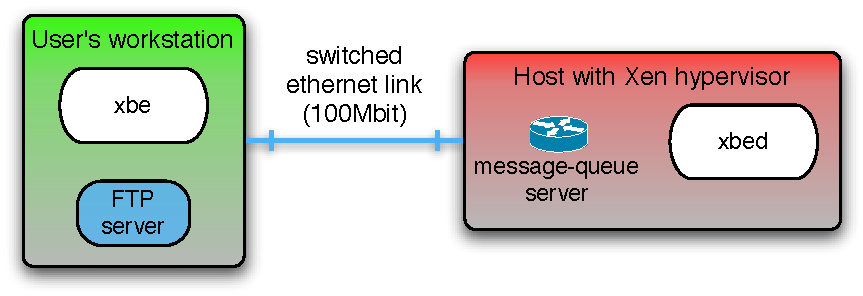
\includegraphics[scale=.55]{experiment-setup}
  \caption[Experimental setup]{The network setup that has been used in the
    experiments.}
  \label{fig:experiment-setup}
\end{figure}

The  only  required  program  on  the  workstation of  the  user  was  the
\emph{xbe} command line tool.  To  keep the setup simple, I also installed
an \gls{glo:FTP}  server on this workstation  machine.  This \gls{glo:FTP}
server delivered  required files for the experiments  (\ie virtual machine
images, input  files, etc.) and  it has also  been used for the  upload of
generated output files.

Basically, both machines are of the same type, but the Xen-host system was
running  in  $32$-bit mode,  while  the  other  one used  $64$-bit.   More
detailed information on the hardware  and operating system of both systems
can be found in Table~\ref{tab:machine-configuration}.

\begin{table}[ht]
  \centering
  \begin{tabular}{@{}lccc@{}}\toprule
                    &                                         & \multicolumn{2}{c}{Xen-host} \\ \cmidrule(lr){3-4}
                    & \multicolumn{1}{c}{Workstation}  & Domain-$0$    & Host \\ \midrule
    Kernel          & \texttt{2.6.19-4-generic-amd64}         & \multicolumn{2}{c}{\texttt{2.6.19-4-server}}   \\
    CPU type        &  AMD Athlon\texttrademark              & \multicolumn{2}{c}{AMD Athlon\texttrademark} \\
    Clock frequency & $2009$~MHz                              & \multicolumn{2}{c}{$2009$~MHz} \\
    CPU count       &  $2$                                    &   $1$    &   $2$ \\
    Main memory     & $2048$~MByte                            &   $512$~MByte   &    $2048$~MByte \\
    \bottomrule
  \end{tabular}
  \caption[Test-environment machine configurations]{Machine configurations of the user's workstation and the Xen-host.}
  \label{tab:machine-configuration}
\end{table}

The next sections  discuss the experiments I have  performed to support my
assumptions about the execution environment,  \ie that it is actually able
to execute  user-provided applications. Each experiment  has been executed
five times and only the average  values of the measured times are shown in
the experiment's  results.  The time  measuring has been performed  by the
job-model implementation --- each time a new state is entered, the current
time is remembered.  These times are then included  in the status messages
as special meta information.

The  first  part shows  some  example executions  such  as  a very  simple
\emph{``Hello  World!''}  execution  or  a more  advanced execution  which
deploys a  website and  provides accessibility to  the virtual  machine by
using an \gls{glo:SSH} server.

The final  part of  this chapter analyzes  the overall performance  of the
\gls{glo:XenBEE}.   In particular,  the influence  on the  total execution
time when using cached or compressed images is studied.

\section{Execution examples}
\label{sec:sample-jobs}

This section  shows you  three example executions  where each one  of them
targets a  different execution scenario.  All experiments  in this section
use the  same virtual machine configuration: $1$  virtual CPU, $128$~MByte
virtual main memory and $256$~MByte swap space.  The operating system that
was used for  the virtual machines is a  stripped-down Ubuntu installation
($450$~MByte)  with  a Xen-aware  Linux  kernel (version  \texttt{2.6.19},
about $8$~MByte in size).

\subsection{Hello World!}
\label{sec:hello-world}

The  first execution  example  is very  simple  --- it  just executes  the
\texttt{echo}  command  with  parameters  that  I supplied  in  a  virtual
machine. The generated  output is then transfered back  to my workstation.
This example is my contribution to the list of implementations that output
the string \texttt{``Hello World!''}.

\begin{figure}[ht]
  \begin{minipage}{0.48\columnwidth}%
    \centering
    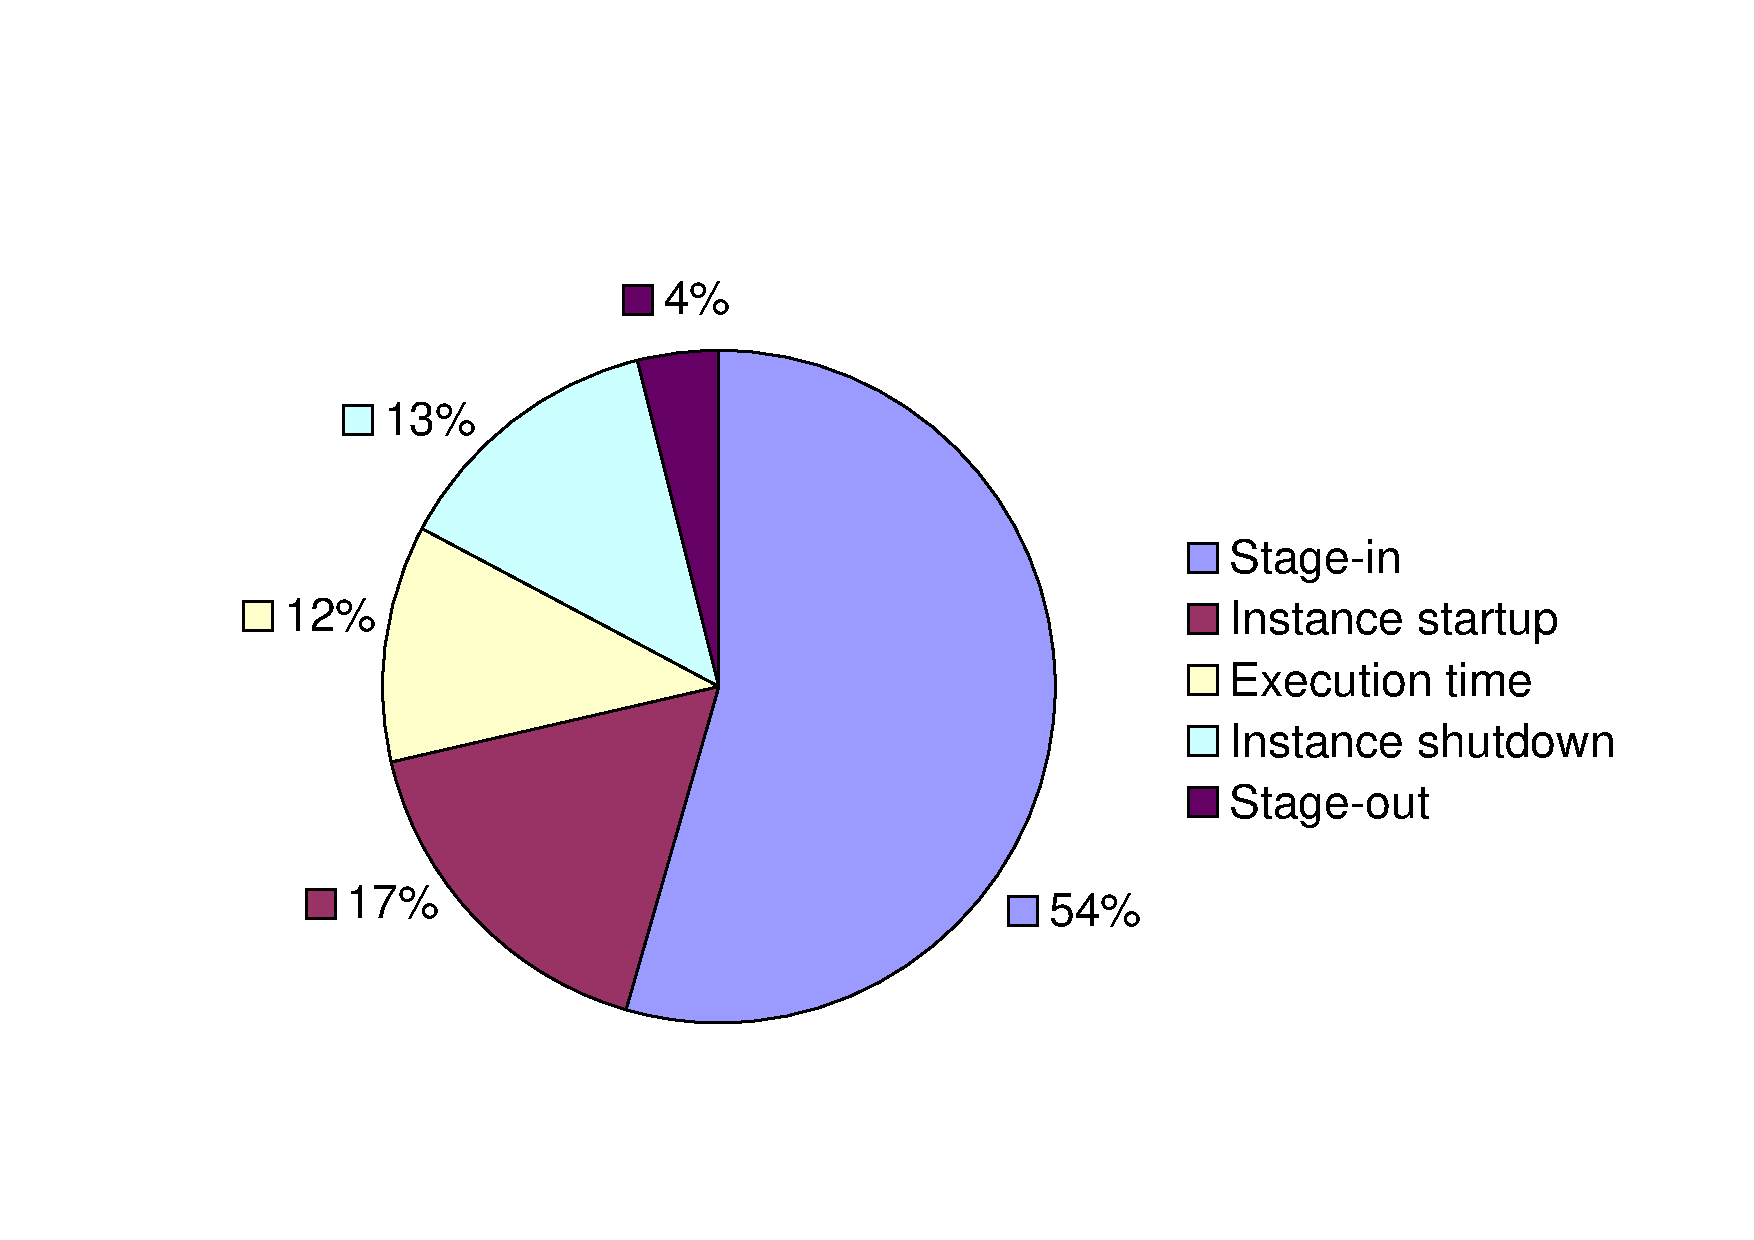
\includegraphics[height=6cm]{results/hello-world}
  \end{minipage}%
  \hfill%
  \begin{minipage}{0.48\columnwidth}%
    \begin{tabular}{@{}lr@{}}\toprule
      Execution step         &   Time ($s$) \\ \midrule % header
      Wait for start message &   $  0.38 $  \\
      Stage-in               &   $ 46.14 $  \\
      Instance startup       &   $ 14.19 $  \\
      Execution time         &   $  9.78 $  \\
      Instance shutdown      &   $ 11.31 $  \\
      Stage-out              &   $  3.21 $  \\
      total                  &   $ 85.01 $  \\ \bottomrule
    \end{tabular}
  \end{minipage}%
  \vspace{1em}
  \caption[Hello  World  example   execution]{Distribution  of  the  total
    execution  time   of  the  \texttt{Hello  World!}   example  over  the
    individual steps.}
  \label{fig:hello-world}
\end{figure}

Figure~\ref{fig:hello-world}  shows the  total execution  time of  the job
broken  down  into  the  times  that  were  spent  in  each  step  of  the
execution. Since the runtime of the program itself is very short --- about
$0.013\ s$ on the workstation --- the overhead introduced by the execution
environment makes up the largest part of the total execution time. Most of
the time  was spent  for transferring  the image and  for starting  up and
shutting down the  virtual machine. The image can  be transferred in about
$38\ s$ from  the workstation to the Xen-host --- the  remaining $8\ s$ of
the Stage-in  step are spent  on setting up  the jail environment  and the
swap  space.  During the  Stage-out  step the  output  of  the program  is
transfered back to  the user's workstation so that I could  have a look at
it.

\subsection{Complex Computation}
\label{sec:complex-example}

The  previous example  was rather  a proof  of concept  execution  than an
actually applicable  execution. A  user would not  want to execute  a job
that  simple and  short with  the overhead  of a  complete  remote virtual
machine. The following  example however could be an  imaginable real world
problem.

In this  case the  user wants  to render various  scenes into  pictures by
using the POV-Ray \cite{POV-Ray}  application. This example relates to the
example       used      in      Section~\ref{sec:req:batch-job-execution},
\nameref{sec:req:batch-job-execution}. Listing~\ref{lst:result:povray-cornell}
shows the important parts of the job description.  The first thing to note
is  the  usage  of  logical  file system  names  (the  \texttt{SPOOL}  for
example).   The first argument  to the  \texttt{povray} executable  is the
scene definition  and the last  argument is the  name of the  output file.
The   stage-in   step  loads   the   \texttt{scene.pov}   file  into   the
\texttt{SPOOL}  directory while  the  stage-out step  takes the  generated
\texttt{scene.png} file and transfers it back to the user.

The  resulting   image\footnote{The  command  line  to   produce  it  was:
  \texttt{povray}     \texttt{+Q11}     \texttt{+A0.01}    \texttt{+W1600}
  \texttt{+H1280} \texttt{+Ocornell.png} \texttt{cornell.pov}} is shown in
Figure~\ref{fig:pov-cornell}.   The virtual  machine image  that  has been
used for this  example was the same as for the  previous example, thus the
times needed to stage in the files in both cases are nearly the same.

\begin{figure}[ht]
  \begin{minipage}{0.48\columnwidth}%
    \centering
    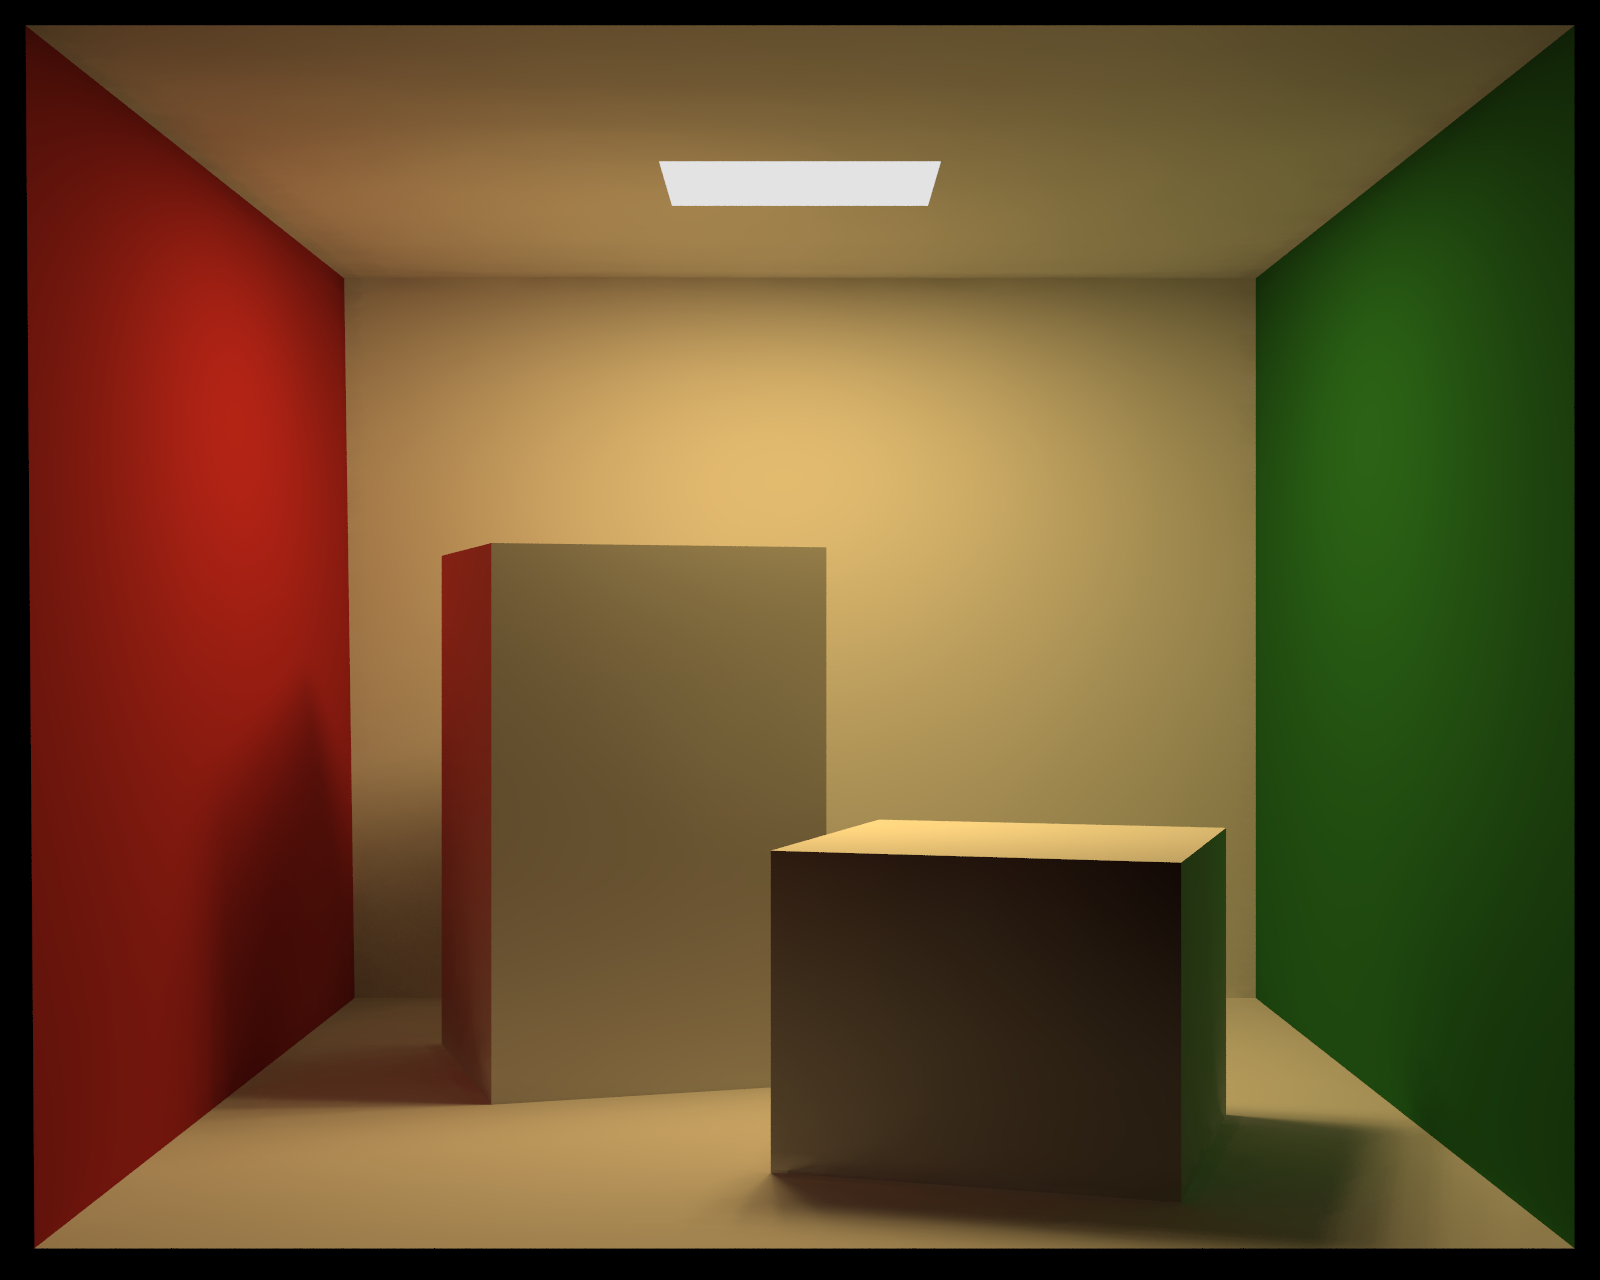
\includegraphics[height=5cm]{results/povray-cornell}
  \end{minipage}%
  \hfill%
  \begin{minipage}{0.48\columnwidth}%
    \begin{tabular}{@{}lr@{}}\toprule
      Execution step         &   Time ($s$) \\ \midrule % header
      Wait for start message &   $   0.50 $ \\
      Stage-in               &   $  47.04 $ \\
      Instance startup       &   $  15.41 $ \\
      Execution time         &   $ 569.81 $ \\
      Instance shutdown      &   $  11.39 $ \\
      Stage-out              &   $   3.36 $ \\
      total                  &   $ 647.51 $ \\ \bottomrule
    \end{tabular}
  \end{minipage}%
  \vspace{1em}
  \caption[POV-Ray  execution result]{The  \texttt{cornell} scene  that is
    included  in the  POV-Ray  program's examples  ---  executed with  the
    \gls{glo:XenBEE}.}
  \label{fig:pov-cornell}
\end{figure}

The execution makes this time use of stage-in and stage-out operations. In
the  stage-in step,  a  scene  description is  loaded  into the  execution
environment.   This  description is  then  passed  to the  \texttt{povray}
executable along  with additional command  line parameters (\eg  to define
the rendering  quality or  the required size  of the output  picture). The
stage-out step  is again  used to retrieve  the generated output  from the
execution environment.

In comparison  to the \emph{Hello World}-example where  the execution time
was barely a fourth of the stage-in time, the execution time outweighs the
stage-in time this time with a  factor of $12$.  If the actual computation
time is just  long enough, the overhead that is  introduced by the virtual
machine preparation gets more  and more insignificant.  The same execution
takes about $406\  s$ when executed directly on  the workstation, thus the
pure execution of the program is still much faster.

\medskip
\begin{center}
  \begin{minipage}{.9\textwidth}
    \begin{lstlisting}[captionpos=b,backgroundcolor=\color{listingcolor},frame=lines,numbers=none,stepnumber=5,numberfirstline=false,numberstyle=\tiny,caption={Important
        parts from the JSDL to describe a \texttt{povray} execution (Note:
        the       listing   does not describe        a       valid       JSDL
        document).},label={lst:result:povray-cornell},language=XML]
<jsdl-posix:POSIXApplication>
  <jsdl-posix:Executable>/usr/bin/povray</jsdl-posix:Executable>
  <jsdl-posix:Argument filesystemName="SPOOL">
    scene.pov
  </jsdl-posix:Argument>
  <!-- quality settings and output redirection omitted -->
  <jsdl-posix:Argument>+Oscene.png</jsdl-posix:Argument>
  <jsdl-posix:WorkingDirectory filesystemName="SPOOL"/>
</jsdl-posix:POSIXApplication> <!-- ... -->
<jsdl:DataStaging>
  <jsdl:FileName>scene.pov</jsdl:FileName>
  <jsdl:Source>
    <jsdl:URI><!-- location of scene file --></jsdl:URI>
  </jsdl:Source>
</jsdl:DataStaging>
<jsdl:DataStaging>
  <jsdl:FileName>scene.png</jsdl:FileName>
  <jsdl:Target>
    <jsdl:URI><!-- destination of result picture--></jsdl:URI>
  </jsdl:Target>
</jsdl:DataStaging>
    \end{lstlisting}
  \end{minipage}
\end{center}

\subsection{Deployment of a Web Server}
\label{sec:deployment-of-a-web-server}

This  example shows  how a  small  web server  can be  deployed using  the
\gls{glo:XenBEE}    ---   it    relates   to    the   example    used   in
Section~\ref{sec:req:server-deployment},
\nameref{sec:req:batch-job-execution}.  The  virtual machine image  can be
generic, \ie it needs only to  contain the web server application and must
make sure that the server gets started during the initialization process.

To  make this  example more  generic,  the content  of the  web server  is
provided as  a stage-in  item as  well.  The content  can for  instance be
staged  in  by  transferring  a  compressed \texttt{tar}  archive  to  the
execution environment. Listing~\ref{lst:result:web-server} shows again the
important  parts  of  the  job   description  that  has  been  used.

\begin{center}
  \begin{minipage}{.9\textwidth}
    \begin{lstlisting}[captionpos=b,backgroundcolor=\color{listingcolor},frame=lines,numbers=none,stepnumber=5,numberfirstline=false,numberstyle=\tiny,caption={File
      system definitions for a web server deployment.},label={lst:result:web-server},language=XML]
<jsdl:Application>
  <xbe:XBEApplication>
    <xbe:ContinuousTask/>
  </xbe:XBEApplication>
</jsdl:Application>
<jsdl:Resources>
  <jsdl:FileSystem name="HOME">
    <jsdl:MountPoint>/root</jsdl:MountPoint>
  </jsdl:FileSystem>
  <jsdl:FileSystem name="WWW">
    <jsdl:MountPoint>/var/www</jsdl:MountPoint>
  </jsdl:FileSystem>
</jsdl:Resources>
<jsdl:DataStaging>
  <jsdl:FileName>.ssh/authorized_keys</jsdl:FileName>
  <jsdl:FilesystemName>HOME</jsdl:FilesystemName>
  <jsdl:Source>
    <jsdl:URI><!-- authorized_keys location --></jsdl:URI>
    <xsdl:Mode>0600</xsdl:Mode>
  </jsdl:Source>
</jsdl:DataStaging>
<jsdl:DataStaging>
  <jsdl:FileName>site.tar.bz2</jsdl:FileName>
  <jsdl:FilesystemName>WWW</jsdl:FilesystemName>
  <jsdl:Source>
    <jsdl:URI><!-- location of content archive --></jsdl:URI>
    <xsdl:Compression algorithm="tbz"/>
  </jsdl:Source>
</jsdl:DataStaging>
    \end{lstlisting}
  \end{minipage}
\end{center}

Since the job defines the deployment of  a server and not a batch job, the
application is  set to the special \texttt{ContinousTask}  provided by the
\gls{glo:XenBEE}. The  description defines  two logical file  systems, the
\texttt{WWW} directory and  the \texttt{HOME} directory.  The \texttt{WWW}
directory is used to specify the location where the web server expects its
contents  and the \texttt{HOME}  directory is  used for  the \gls{glo:SSH}
login that I will describe in a moment.

The complete  content (\ie  directories and files)  for the web  server is
stored in a compressed \texttt{tar}  archive. This file is staged into the
\texttt{WWW}  directory  and  the  \emph{xbed}  decompresses  it  at  this
specific location --- note the usage of the compression algorithm.

To  be  able  to  change  the  content  or  to  modify  the  web  server's
configuration after the  virtual machine has been started,  I installed an
\gls{glo:SSH} server into the image as well.  The \gls{glo:SSH} server was
configured to  allow access only by public-key  authorization.  Thus there
was   an   additional   staging   operation  required   which   loads   an
\texttt{authorized\_keys} file into the  virtual machine.  Due to security
reasons,  the \gls{glo:SSH}  server requires  that this  file can  only be
accessed by the  user himself --- the special  \texttt{Mode} element takes
care of that.

I submitted  the job to  the \emph{xbed} and  after about $60\ s$  the web
server was running. The address of  the virtual machine is included in the
status message, so I could point  my web browser to the address and browse
through the deployed content.

\section{Performance Analysis}

The  previous  section  showed  that  a considerable  part  of  the  total
execution time  is spent in the  Stage-in step. This  section will analyze
this step in more detail.  Two different approaches that could improve the
execution time are discussed as well.

The bare  execution time  of a  job cannot be  decreased by  the execution
environment as  such, because it  mainly depends on the  implementation of
the virtualization back-end and the hardware that is being used.  The only
step in the  execution path that can effectively  be modified and improved
is the stage-in process.

The current  implementation of the \gls{glo:XenBEE} offers  two options to
improve that part, \emph{compression}  and \emph{caching} of user supplied
files.  The following sections deal with those two possibilities.

\subsection{Compressed Images}
\label{sec:compression}

The experimental setup uses the POV-Ray raytracer to render a picture, but
this time a less time consuming configuration\footnote{The execution takes
  about $60\ s$ on a virtual machine and only $21\ s$ on the workstation.}
has been used.   The same image as in the previous  examples is used.  The
uncompressed image has a size  of $449$~MByte that can be transferred from
the  workstation to the  Xen-host in  about $41\  s$ (assuming  an average
throughput of  $11$~MByte/$s$).  The  $449$~MByte image can  be compressed
with the \texttt{bzip2}  program\footnote{I applied the \texttt{-3} option
  to \texttt{bzip2}  to get a  faster compression/decompression behavior.}
to a  $145$~MByte sized file  which can be  transferred in about  $13\ s$.
Figure~\ref{fig:compression-comparison-small}  shows  the distribution  of
the total execution time on the individual steps.

\begin{figure}[ht]
  \subfigure[Uncompressed image ($450$~MByte)]{
    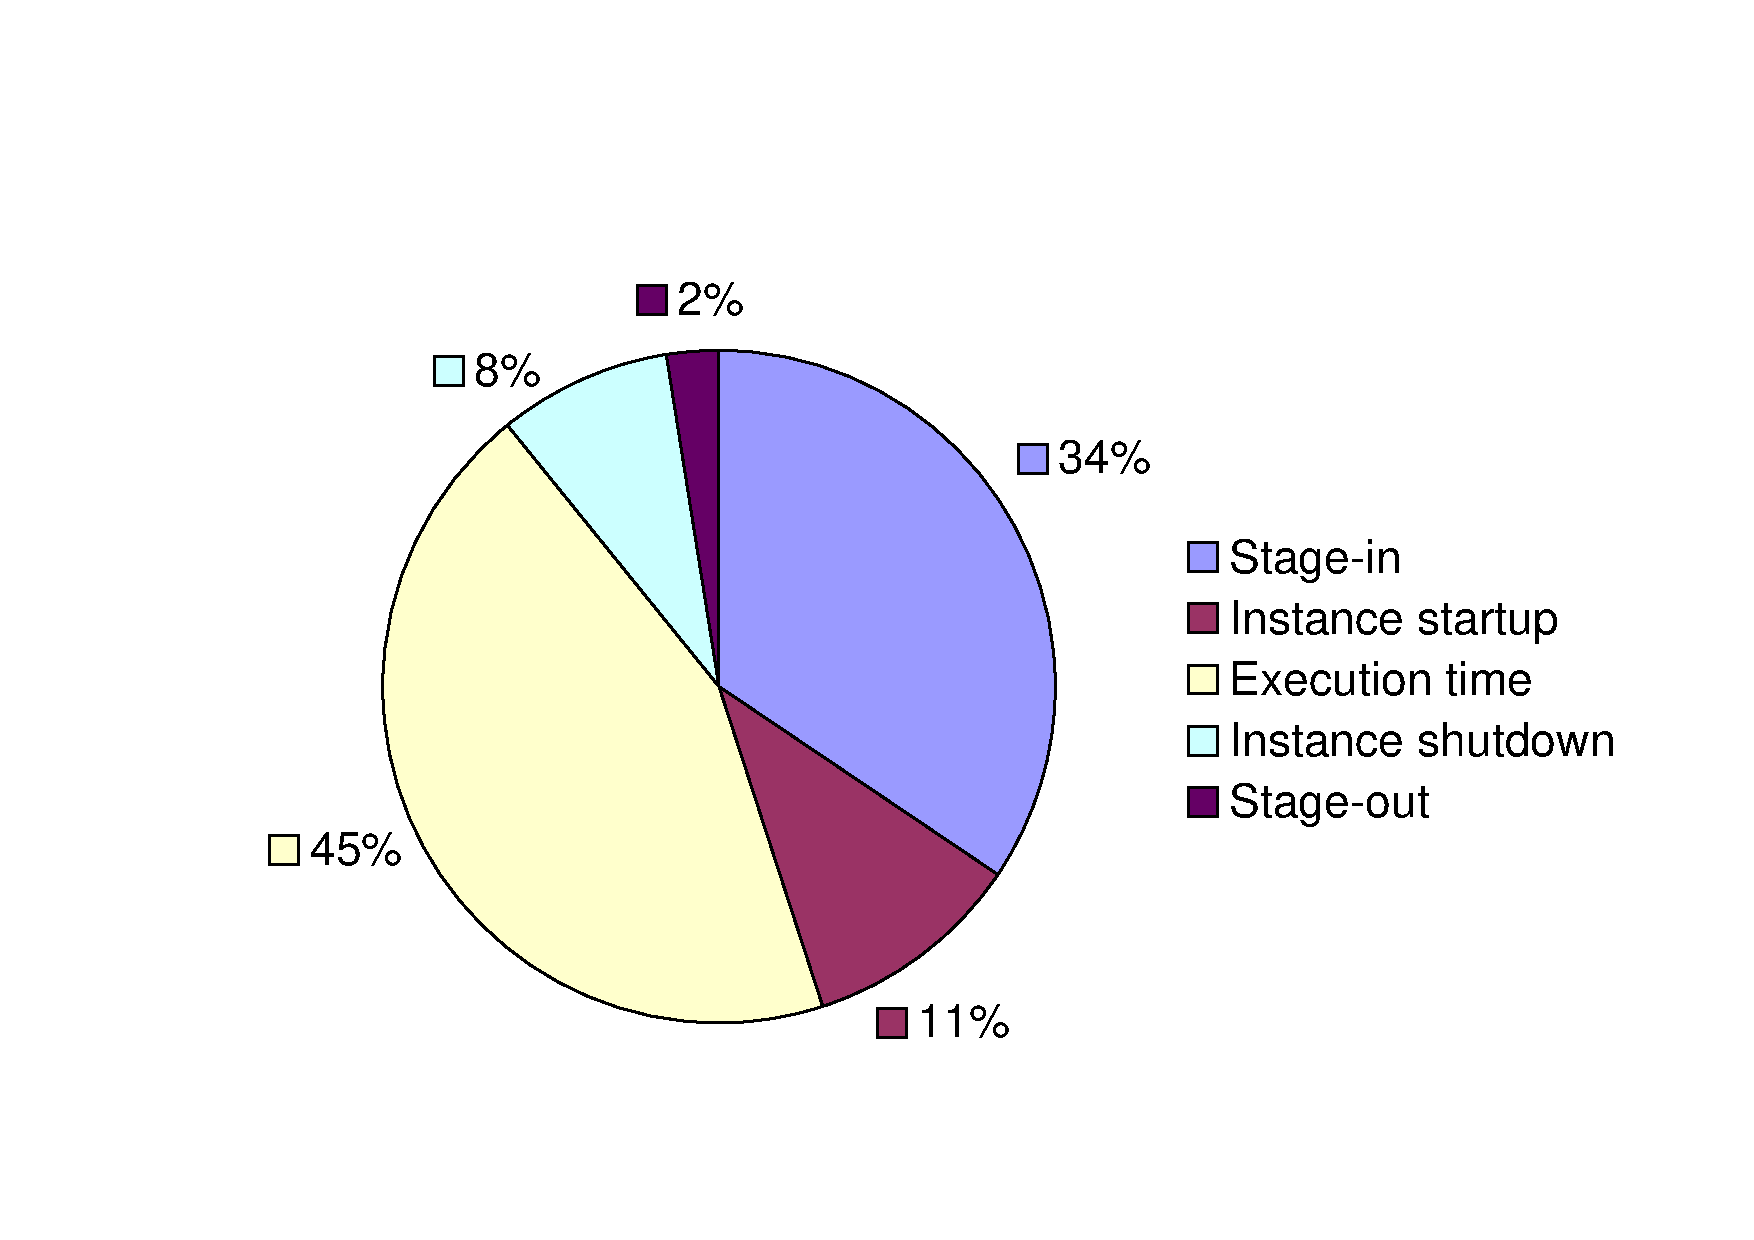
\includegraphics[width=.45\textwidth]{results/uncompressed-small}
  }
  \subfigure[Compressed image ($145$~MByte)]{
    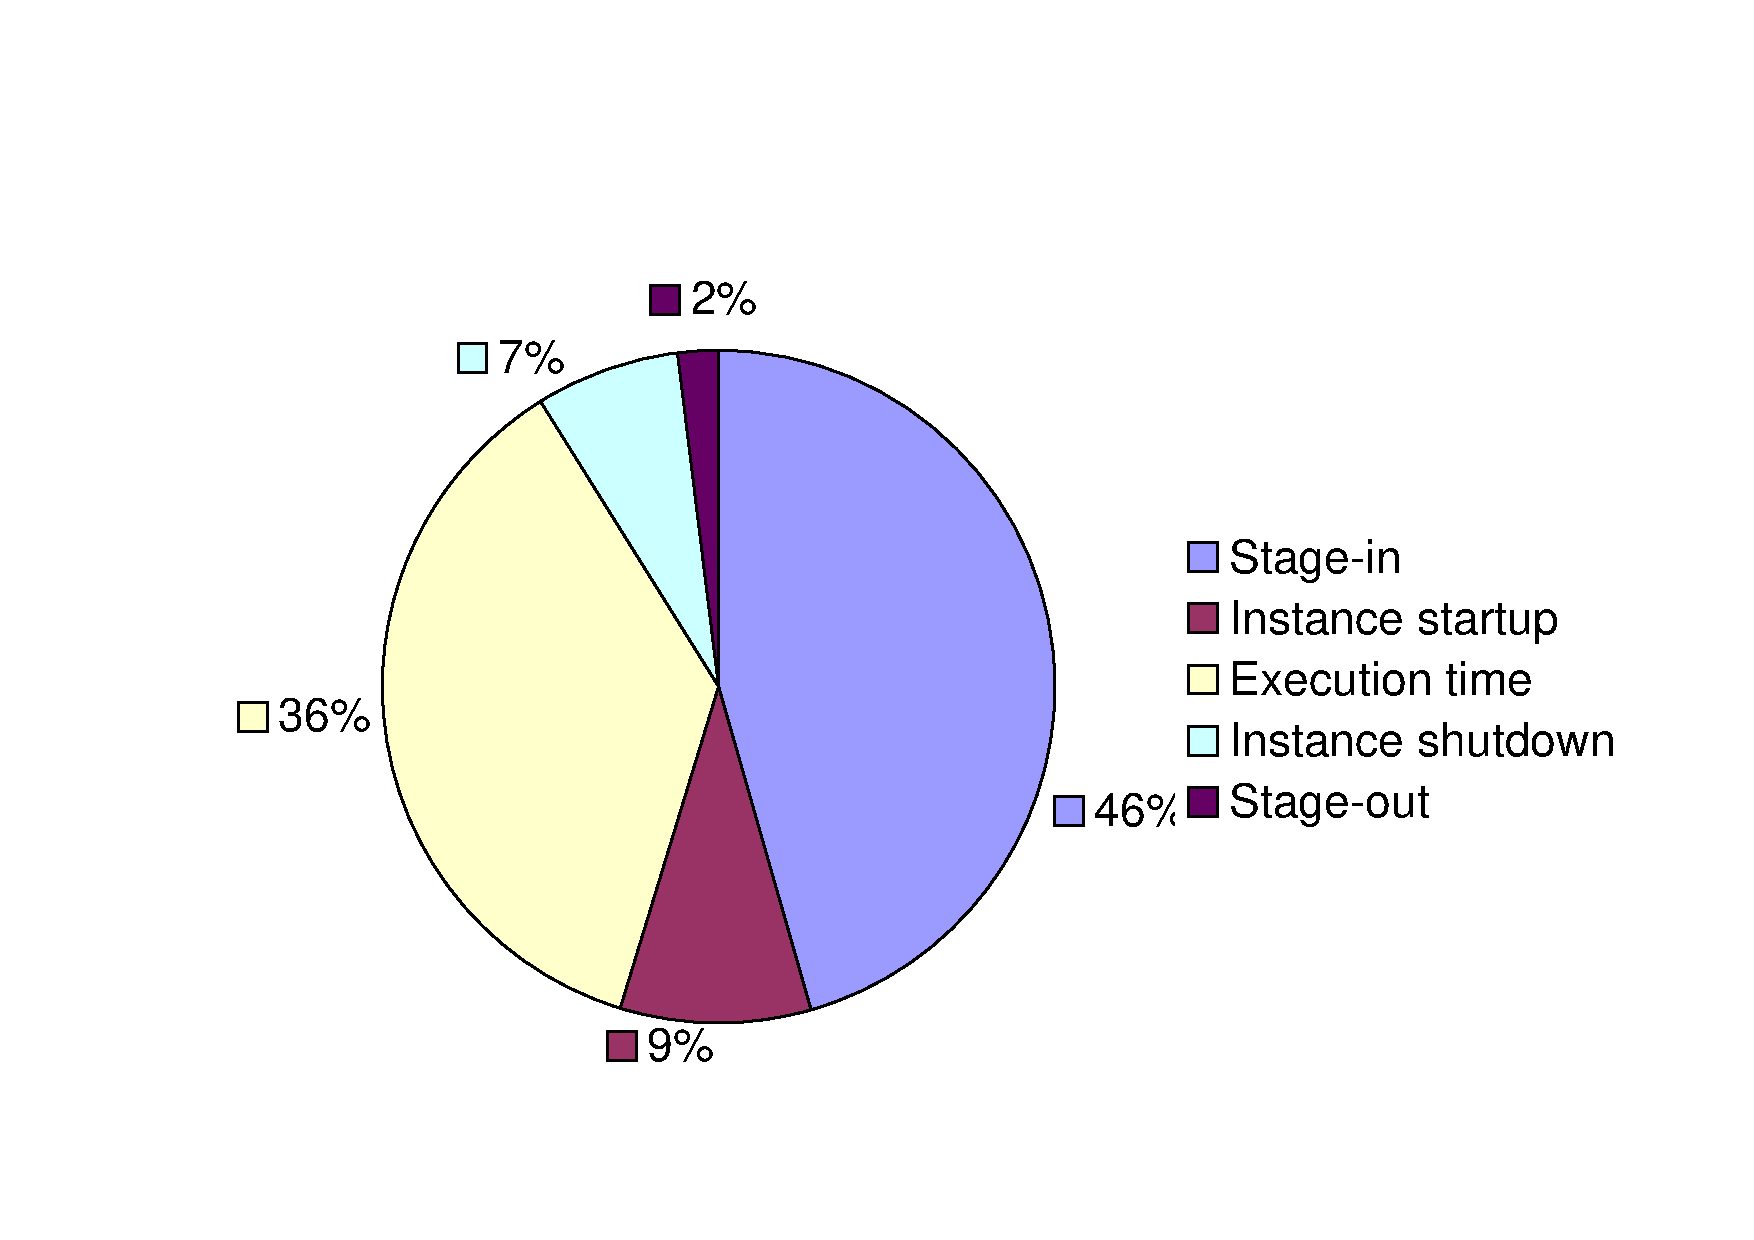
\includegraphics[width=.45\textwidth]{results/compressed-small}
  }
  \label{fig:compression-comparison-small}
  \caption[Uncompressed   \vs  compressed   small   images]{Comparison  of
    uncompressed/compressed images (small image).}
\end{figure}

Surprisingly, the total execution time of  the job had not decreased, as I
thought.   The  execution  time  had  even increased  by  circa  $30\  s$.
Table~\ref{tab:compression-comparison-small}  shows the  exact  times that
have been measured,  it also shows that the  main divergence occurs during
the  Stage-in  process.  The  transfer  of  the  compressed image  can  be
accomplished in  about $12\  s$, but the  complete Stage-in  step consumed
$74.55\  s$.   That  means,  circa   $60\  s$  have  been  spent  for  the
decompression of  the image.  The  decompression alone consumes  more time
than the transfer of the uncompressed image which took only $46.24\ s$.

\begin{table}[ht]
  \centering
  \begin{tabular}{@{}lrr@{}}\toprule
                      & \multicolumn{2}{c}{Time ($s$)} \\ \cmidrule(lr){2-3}
    Execution step         &  uncompressed      & compressed \\ \midrule % header
    Wait for start message &  $   0.40 $        & $   0.40 $    \\
    Stage-in               &  $  46.24 $        & $  74.55 $    \\
    Instance startup       &  $  14.20 $        & $  14.94 $    \\
    Execution time         &  $  59.65 $        & $  59.68 $    \\
    Instance shutdown      &  $  11.29 $        & $  11.29 $    \\
    Stage-out              &  $   3.21 $        & $   3.25 $    \\
    total                  &  $ 134.99 $        & $ 164.11 $    \\
    \bottomrule
  \end{tabular}
  \caption[Uncompressed \vs compressed small images]{Comparison of the execution times when using uncompressed or
    compressed images, $450$~MByte and $145$~MByte respectively.}
  \label{tab:compression-comparison-small}
\end{table}

This example  used an image that  was mostly filled with  data.  A typical
usage scenario for  the \gls{glo:XenBEE} would however be  to use a sparse
image, \ie an image that  is mostly empty. The following execution example
uses an  image with $8$~GByte  of total size  but only about  $1$~GByte is
actually  used.   Compressing  this  image  results  in  a  file  that  is
$499$~MByte large. Both  files can be transferred from  the workstation to
the Xen-host in  circa $745\ s$ and $45\ s$ respectively.   In order to be
faster, the decompression has a time buffer of $700\ s$.

\begin{figure}[ht]
  \subfigure[Uncompressed image ($8$~GByte)]{
    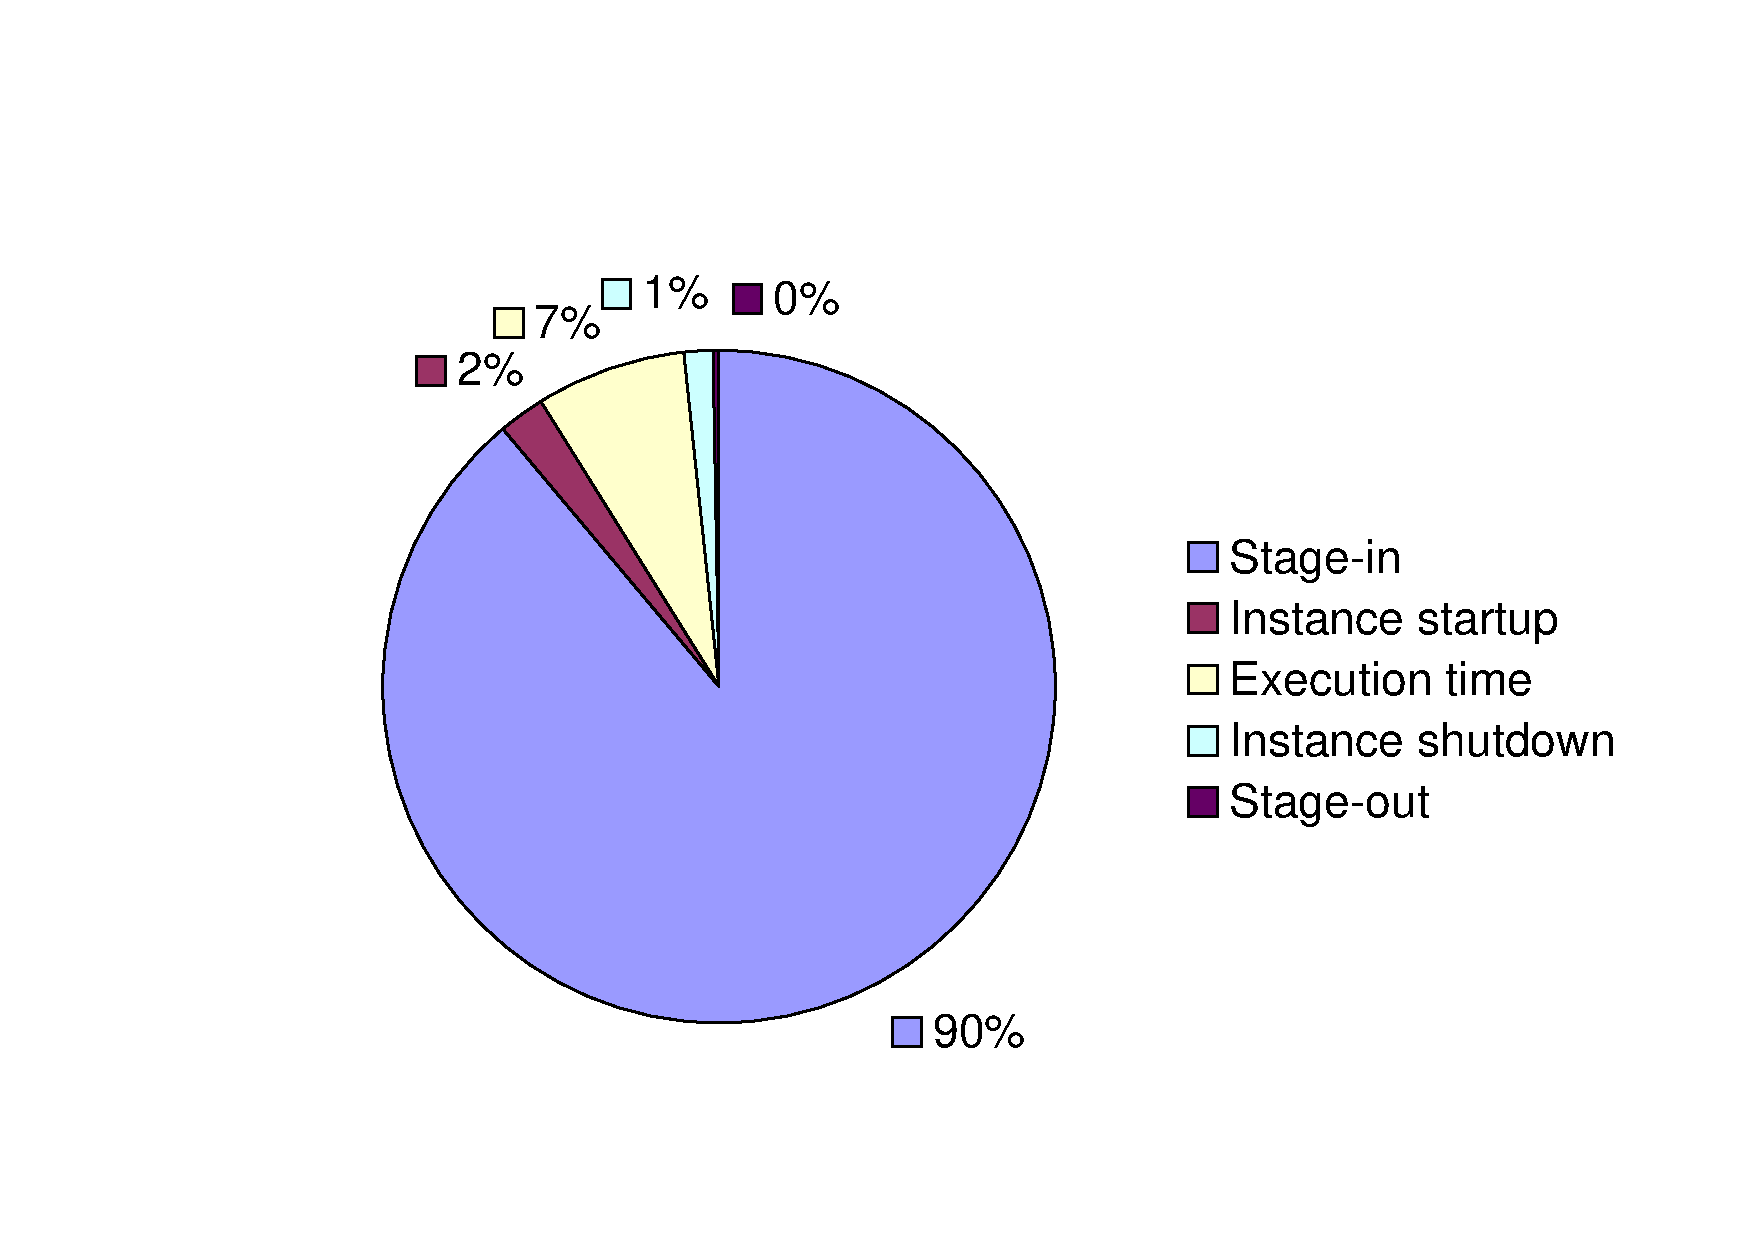
\includegraphics[width=.45\textwidth]{results/uncompressed-big}
  }
  \subfigure[Compressed image ($499$~MByte)]{
    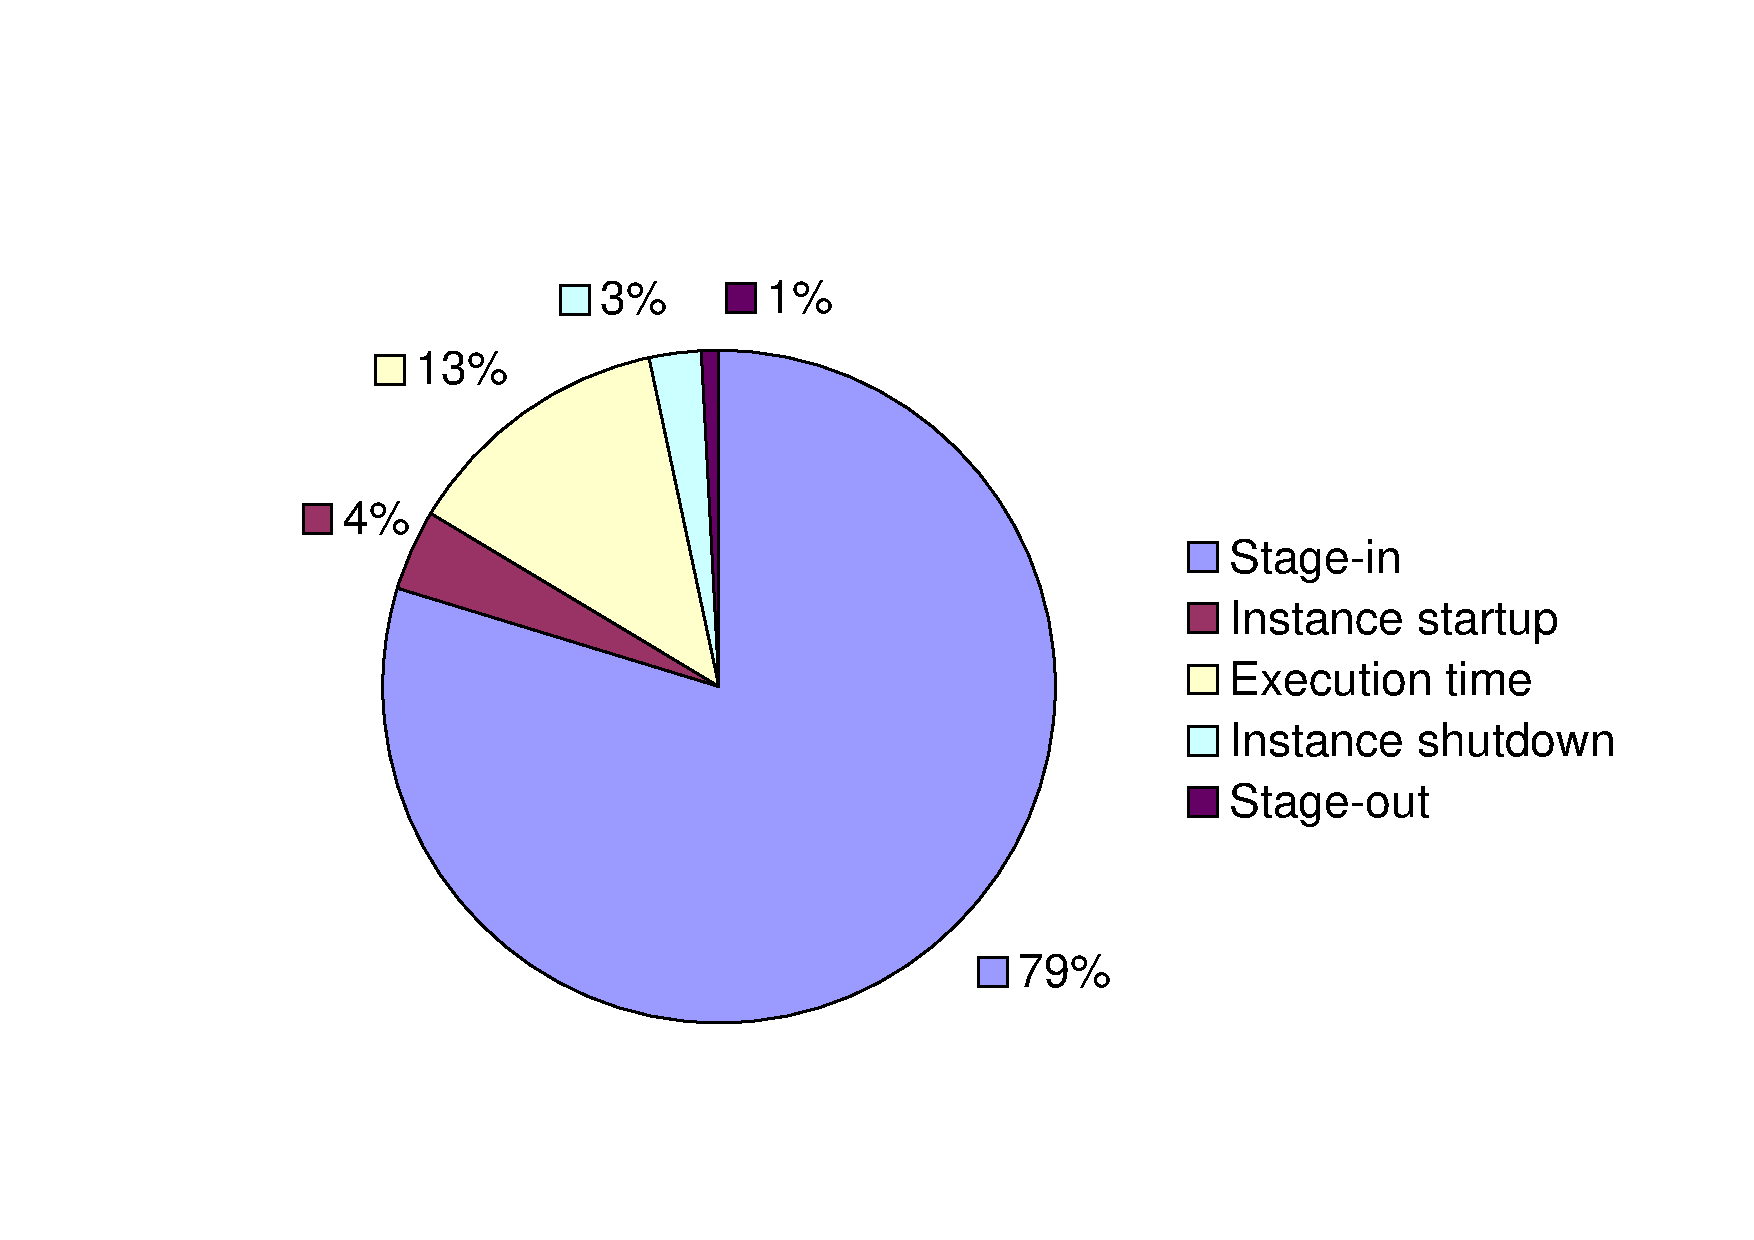
\includegraphics[width=.45\textwidth]{results/compressed-big}
  }
  \label{fig:compression-comparison-big}
  \caption[Uncompressed \vs compressed large images]{Comparison of uncompressed/compressed images (large image).}
\end{figure}

This time  the usage  of a compressed  image outperforms  the uncompressed
variant significantly. The time consumption distribution on the individual
steps        of       both        variants        is       shown        in
Figure~\ref{fig:compression-comparison-big}. Due to  the difference of the
total  execution  times,  the  diagram  does  not  clearly  visualize  the
improvement.  The  exact timings  that were used  to generate  diagram are
shown  in   Table~\ref{tab:compression-comparison-big}.   Staging  in  the
compressed image is twice as fast as staging in the uncompressed image and
the  overall  execution time  dropped  to  circa  $55\%$ of  the  original
execution time.

\begin{table}[ht]
  \centering
  \begin{tabular}{@{}lrr@{}}\toprule
                      & \multicolumn{2}{c}{Time ($s$)} \\ \cmidrule(lr){2-3}
    Execution step         &  uncompressed      & compressed \\ \midrule % header
    Wait for start message &   $   0.45 $       & $   0.50 $    \\
    Stage-in               &   $ 729.72 $       & $ 359.18 $    \\
    Instance startup       &   $  17.60 $       & $  17.70 $    \\
    Execution time         &   $  58.49 $       & $  58.51 $    \\
    Instance shutdown      &   $  11.36 $       & $  11.41 $    \\
    Stage-out              &   $   3.38 $       & $   3.41 $    \\
    total                  &   $ 821.00 $       & $ 450.71 $    \\
    \bottomrule
  \end{tabular}
  \caption[Uncompressed \vs compressed large images]{Comparison of uncompressed/compressed images (large image).}
  \label{tab:compression-comparison-big}
\end{table}

\subsection{Data Caching}
\label{sec:data-caching}

The  caching  of  data can  always  be  used  but  the gain  in  execution
performance  is greatest  when the  cached data  is used  fairly  often. A
virtual machine image that contains  one or more applications that will be
used by  several users  for many  job executions should  be cached  on the
server  side, since the  transfer rate  is boosted  nearly to  the maximal
reachable  rate.

Currently,  the  cache   is  implemented  by  storing  the   data  on  the
Xen-host. Using  a cached file therefore  means, that it has  to be copied
into the task's spool directory. The  upper bound of the transfer rate for
the network connection, as well as  for the internal cache is thus limited
by  the  writing performance  of  the  file system  that  is  used on  the
Xen-host. I determined  this performance on the Xen-host  with a benchmark
tool    called     \texttt{bonnie++}\footnote{The    homepage    of    the
  \texttt{bonnie++}     benchmark     tool     can     be     found     at
  \url{http://www.coker.com.au/bonnie++/}}.   The   determined  pure-write
performance on the Xen-host was  about $40$~MByte/$s$ which is nearly four
times     faster     than      the     average     network     throughput.
Figure~\ref{fig:pov-cache-comparison-short}  shows the  gain  of execution
performance when  using a cached image  for the same job  execution as for
the non-caching variant.

\begin{figure}[ht]
  \subfigure[POV-Ray example without cache]{
    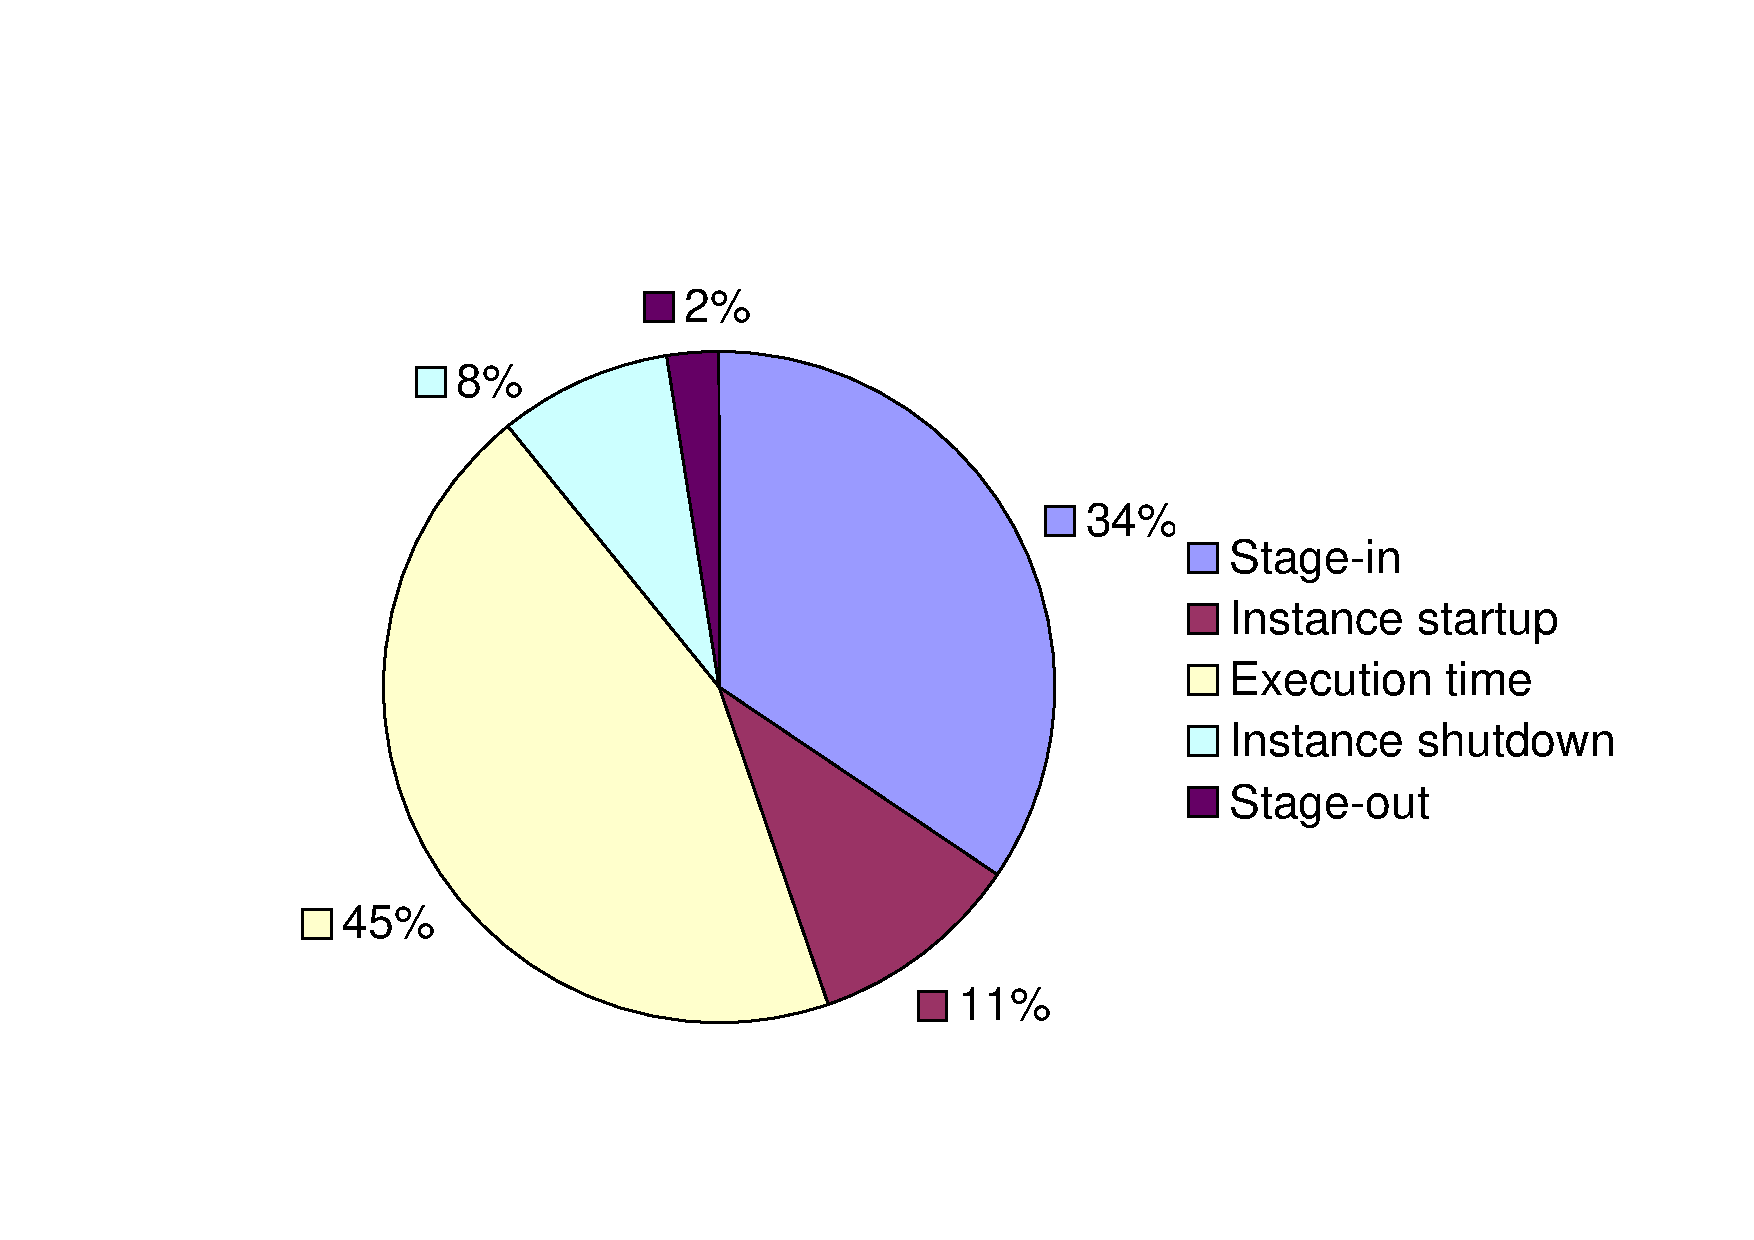
\includegraphics[width=.45\textwidth]{results/cache-fast-nocache}
  }
  \subfigure[POV-Ray example with cached image]{
    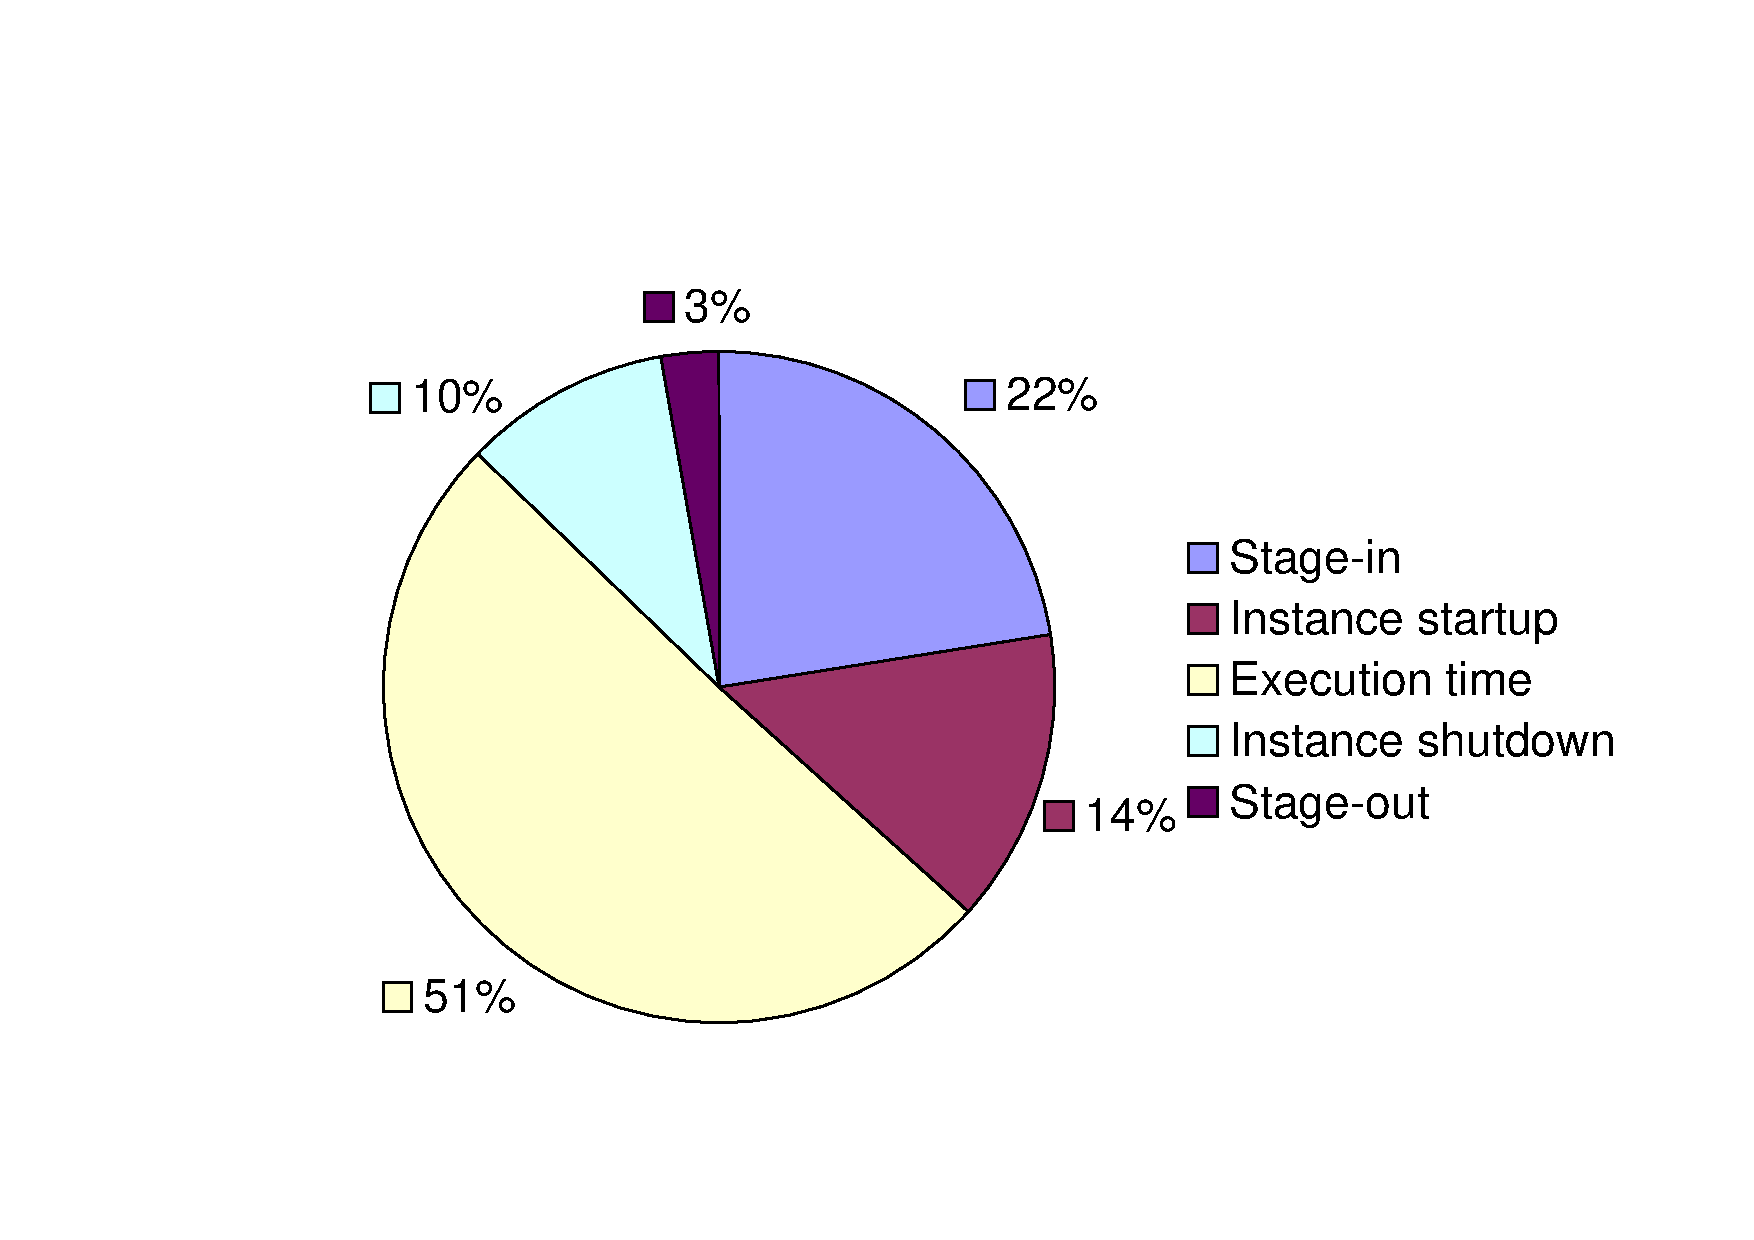
\includegraphics[width=.45\textwidth]{results/cache-fast-cache}
  }
  \caption[Not cached  \vs cached  images]{Comparison of POV-Ray  job with
    and without cache usage.}
  \label{fig:pov-cache-comparison-short}
\end{figure}

The stage-in of the cached image  should have taken about $16\ s$ provided
that the  file is written in $10\  s$ and eventually set  up after another
$6\ s$. The additional $6\ s$  are due the jail environment setup. But the
actual  time required  to  stage in  the  virtual machine  files was  only
reduced             by            about             $45\%$            (see
Table~\ref{tab:povray-nocache-cache-comparision-short}   for   the   exact
values). This may be explained by the  fact that the cached file had to be
read  and written  from  the  same physical  device.

\begin{table}[ht]
  \centering
  \begin{tabular}{@{}lrr@{}}\toprule
                           &    \multicolumn{2}{c}{Time ($s$)} \\ \cmidrule(lr){2-3}
    Execution step         &  no cache          & cached image \\ \midrule % header
    Wait for start message &   $   0.42 $       & $   0.41  $    \\
    Stage-in               &   $  46.22 $       & $  25.68  $    \\
    Instance startup       &   $  14.14 $       & $  16.24  $    \\
    Execution time         &   $  59.79 $       & $  58.15  $    \\
    Instance shutdown      &   $  11.28 $       & $  11.30  $    \\
    Stage-out              &   $   3.20 $       & $   3.22  $    \\
    total                  &   $ 135.05 $       & $ 115.00  $    \\
   \bottomrule
 \end{tabular}
 \caption[Not cached \vs cached images]{Comparison of the execution step times of the POV-Ray example without and with using a
   cached image.}
 \label{tab:povray-nocache-cache-comparision-short}
\end{table}

\subsection{Conclusions}

The  shown example  executions always  made  use of  rather large  virtual
machine image, but it could also  be thinkable to use very small images to
provide ``instant  virtual machines''.

Since the \emph{xbeinstd} must be  installed in the virtual machine image,
a complete  Python installation has to  be installed as  well.  The Python
libraries, as  well as the required \texttt{twisted}  framework need about
$25$~MByte. With some work an image  could be created that needs less than
$100$~MByte and  still can  contain an application  that does  not require
large input files.   Virtual machines using such images  could be deployed
in about  half a minute. Unfortunately, I  could not come up  with such an
image in time, so that I cannot provide time measurements.

My conclusions of  the performance analysis is to use  caching as often as
it  is possible  and compression  only when  sparse files  are  used.  The
caching of an  image does not make  sense if the image is  used only once,
because it  still has to  be transferred to  the Xen-host prior it  can be
used. But if  the image will be  reused over and over again,  it should be
cached.

Compressed  images can  always be  used  if the  transfer time  has to  be
reduced at all  costs. This may involve that  the complete execution takes
longer than the  ordinary execution with a raw image.   On the other hand,
if the image is sparse,  compression can provide a significant speed-up of
the execution time.

Both techniques can be used simultaneously  to get the best of both worlds
(\ie caching of compressed images).


% \begin{itemize}
% \item same execution takes on the workstation $406\ s$
% \end{itemize}

% \begin{figure}[ht]
%   \subfigure[POV-Ray example without cache]{
%     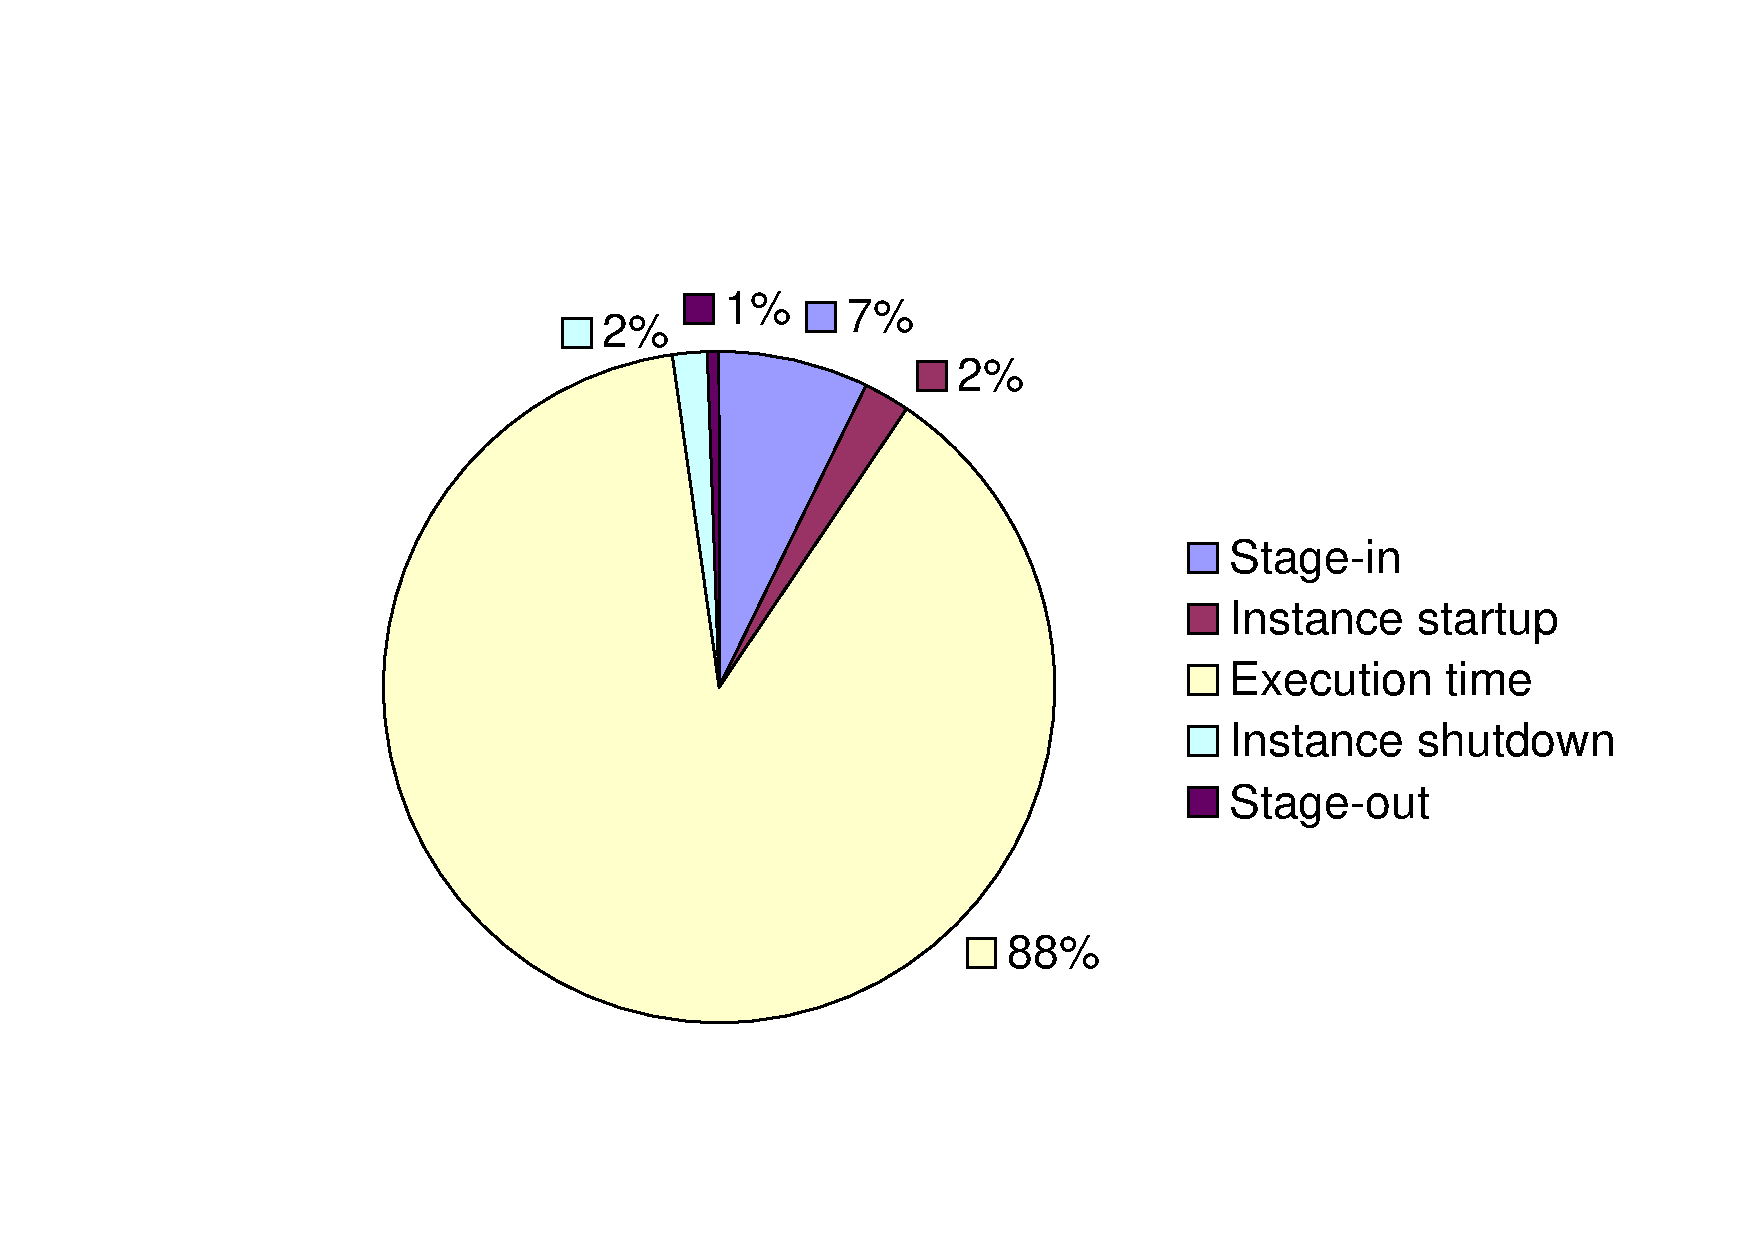
\includegraphics[width=.45\textwidth]{results/povray-nocache}
%   }
%   \subfigure[POV-Ray example with cached image]{
%     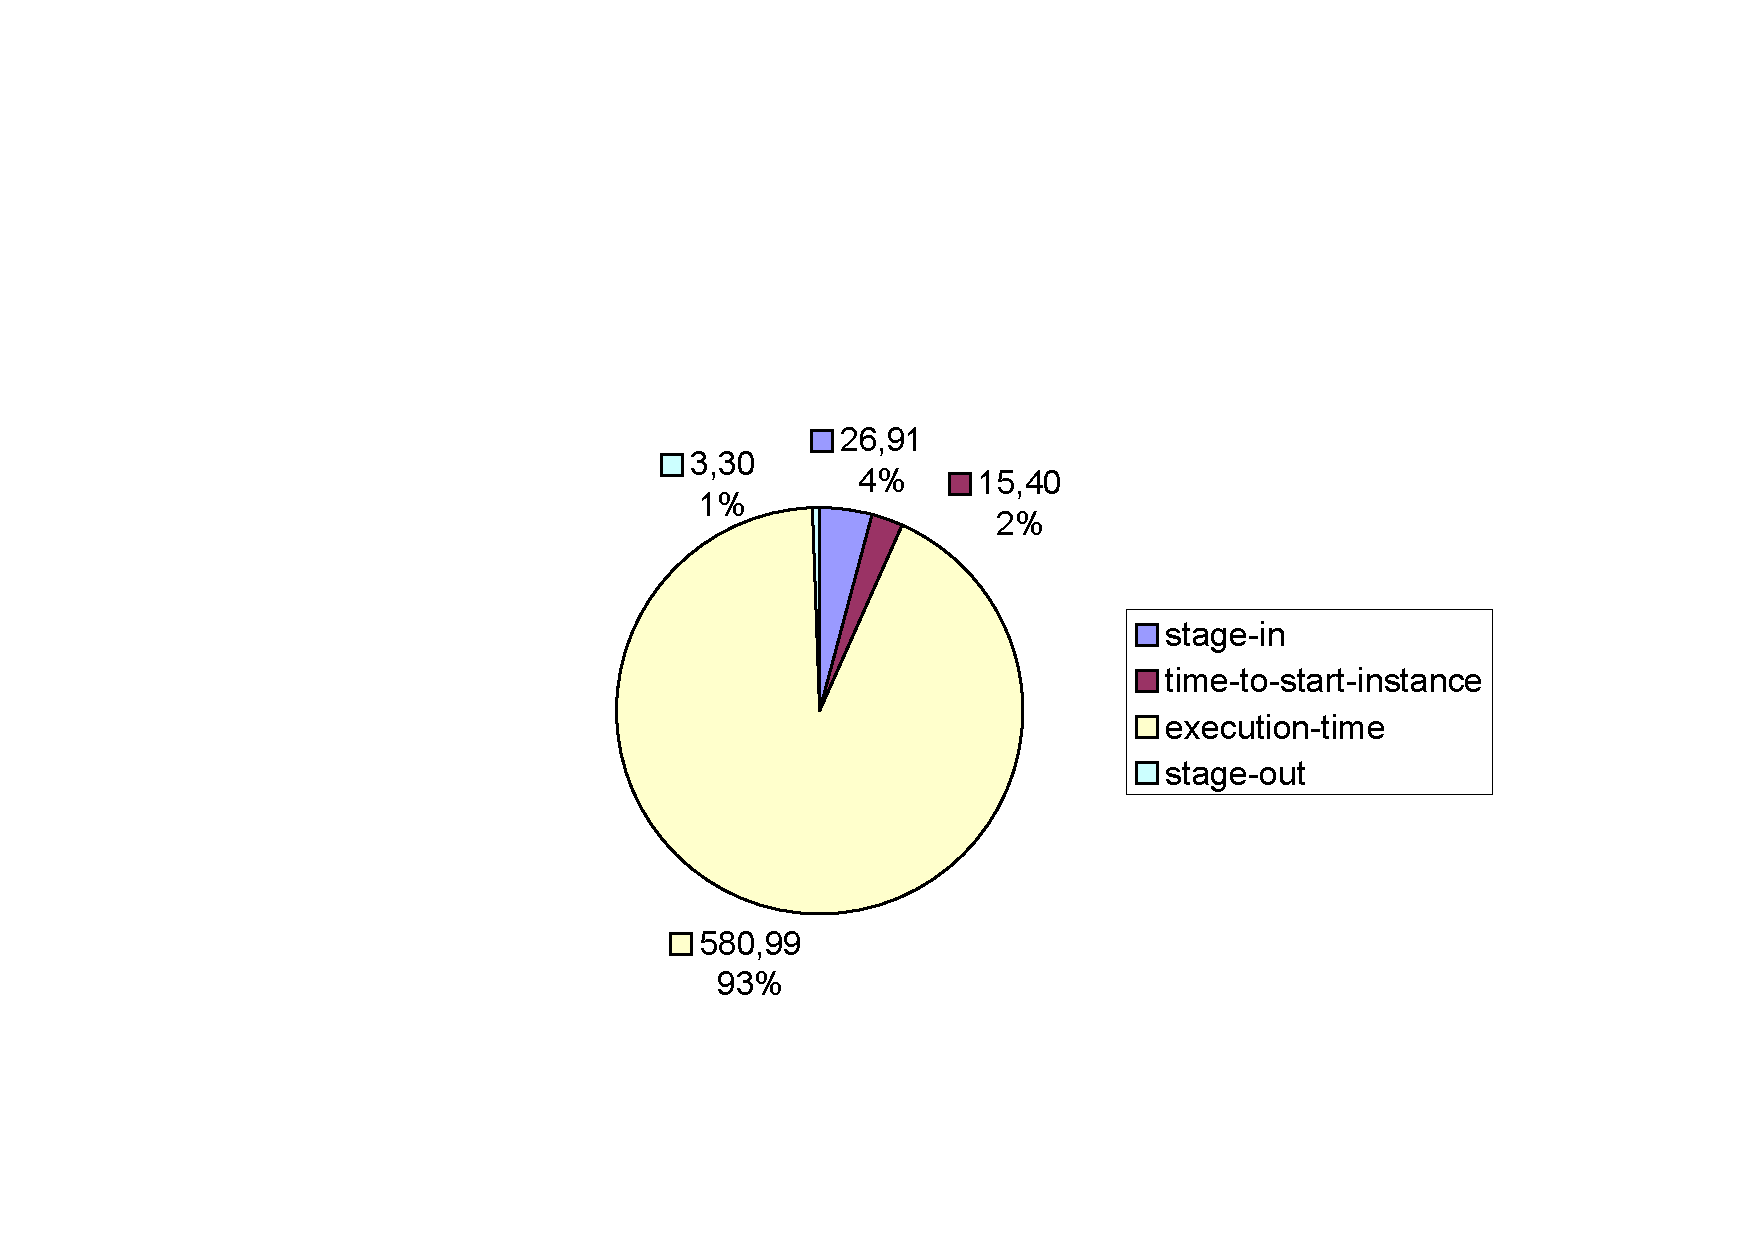
\includegraphics[width=.45\textwidth]{results/povray-cache}
%   }
%   \caption[Not cached \vs  cached images (long execution time)]{Comparison
%     of POV-Ray job with and without cache usage (long execution time).}
%   \label{fig:pov-cache-comparison-long}
% \end{figure}

% \begin{table}[ht]
%   \centering
%   \begin{tabular}{@{}lrr@{}}\toprule
%                            &    \multicolumn{2}{c}{Time ($s$)} \\ \cmidrule(lr){2-3}
%     Execution step         &  no cache          & cached image \\ \midrule % header
%     Wait for start message &   $   0.41 $       & $   0.41 $    \\
%     Stage-in               &   $  46.32 $       & $  26.24 $    \\
%     Instance startup       &   $  14.15 $       & $  16.25 $    \\
%     Execution time         &   $ 569.57 $       & $ 568.09 $    \\
%     Instance shutdown      &   $  11.29 $       & $  11.39 $    \\
%     Stage-out              &   $   3.31 $       & $   3.31 $    \\
%     total                  &   $ 645.05 $       & $ 625.69 $    \\
%     \bottomrule
%   \end{tabular}
%   \caption[Not cached \vs cached images (long execution time)]{Comparison of the
%     execution step times of the POV-Ray example without and with using a
%     cached image (long execution time).}
%   \label{tab:povray-nocache-cache-comparision-long}
% \end{table}


%%% Local Variables: 
%%% mode: latex
%%% TeX-master: "main"
%%% End: 
